%!TEX root = ../../main.tex


\begin{figure}[!htb]
\centering
%\hrulefill\\
%\vspace{5pt}
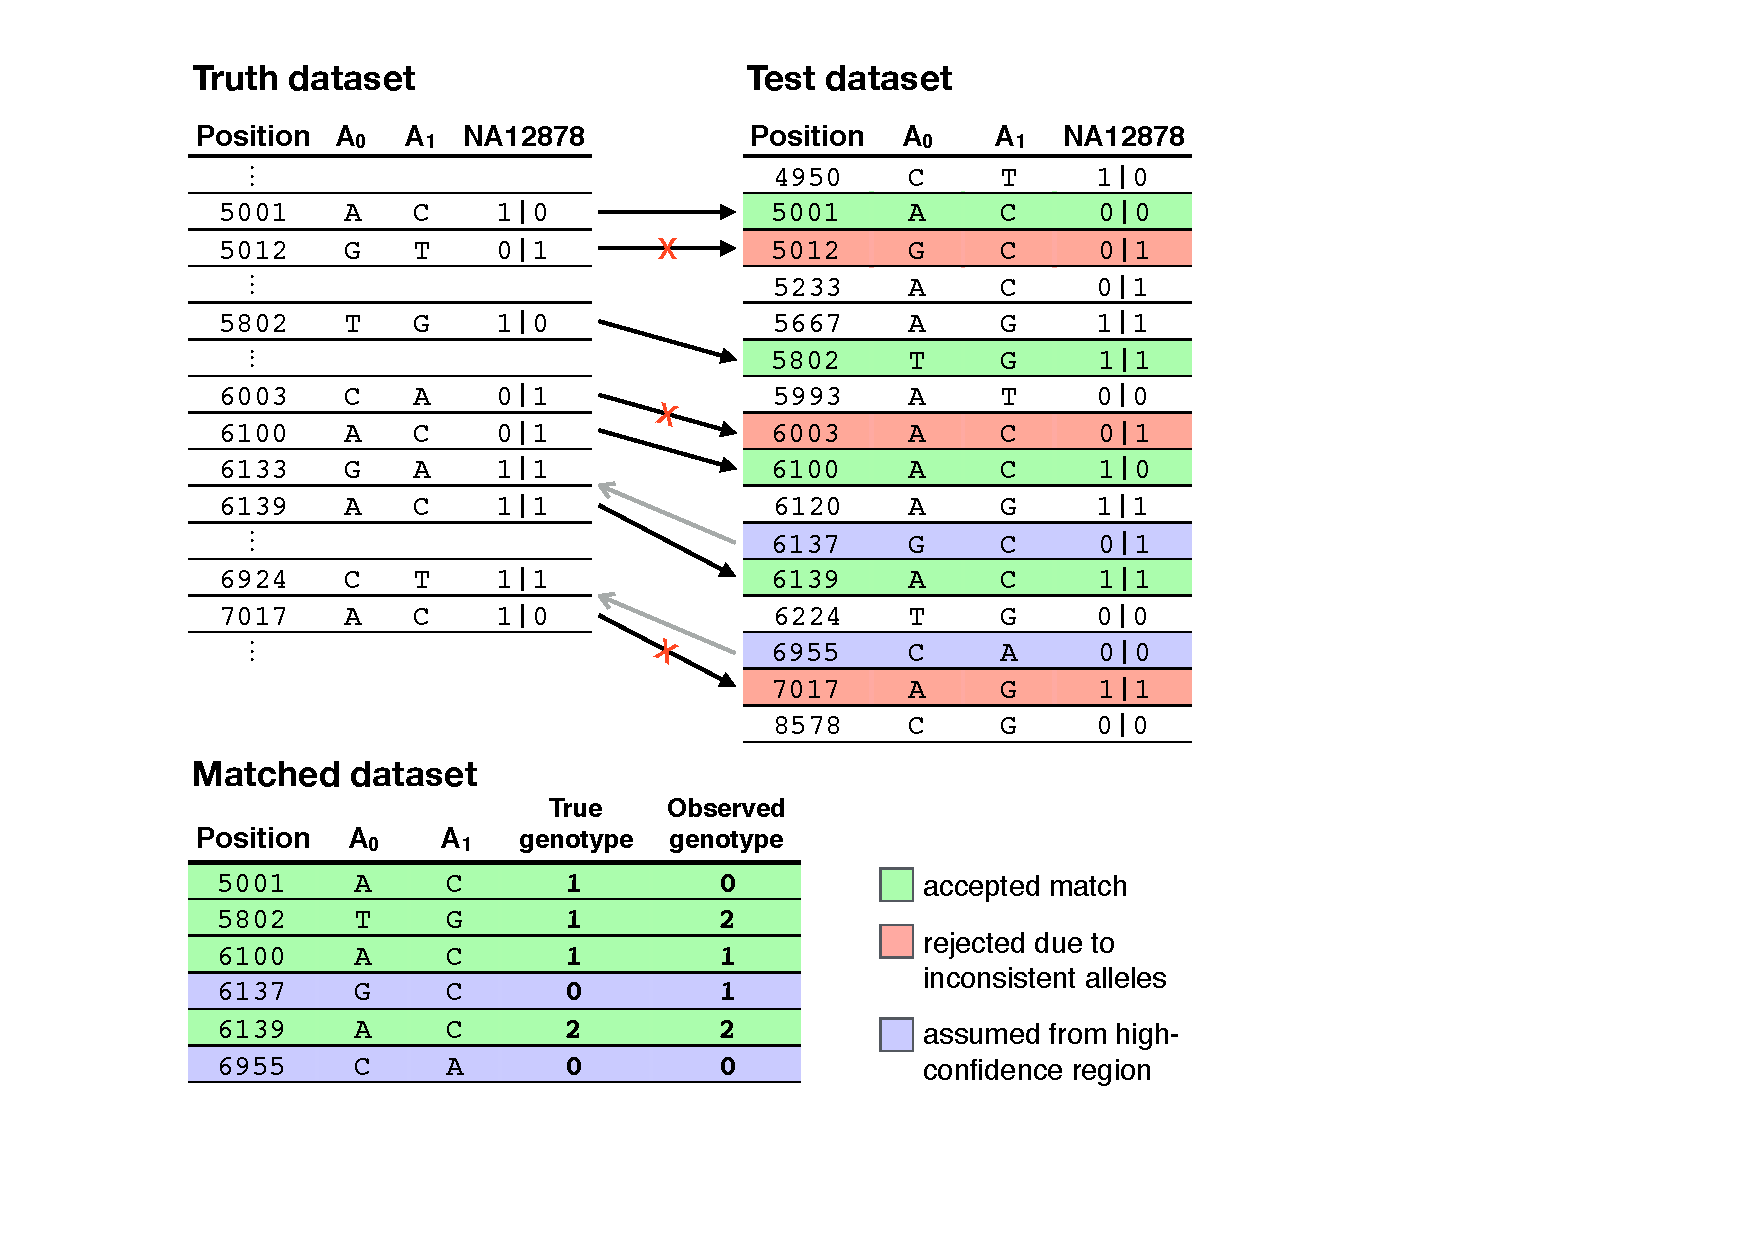
\includegraphics[width=0.666\textwidth]{./img/ch4/info_errormatch}
\Caption{Illustration of the matching process in the generation of error profiles}
{Variant data were reduced to \glspl{snp} and matched per chromosome by variant position and both alleles ($A_0$ and $A_1$) as recorded for either \texttt{NA12877} or \texttt{NA12878}.
Gaps shown in the truth dataset indicate the regions removed after filtering using the accessibility mask provided by \gls{ipg}, such that only high confidence variant calls were retained.
Note that the truth dataset did not contain \glspl{snp} homozygous for the reference allele, but which were assumed from high-confidence regions if present in the test dataset.
This is indicated by left-pointing arrows.}
{fig:info_errormatch}
% \vspace{-5pt}
% \hrulefill%
\end{figure}
